\documentclass{article}

\usepackage{style/preamble}
\usepackage{style/mytikz}
\usepackage{parskip}

\newcounter{dip}

\begin{document}
  \title{Problem Set 3 - Riemann--Hurwitz}
  \date{}
  \maketitle


For today, let $X$ and $Y$ be compact connected Riemann surfaces with atlases $(U_i, \varphi_i)$ and $(V_j,\psi_j)$, respectively, and let $f: X \rightarrow Y$ be a non-constant complex differentiable function between them.








\section{Ramified coverings of Riemann surfaces}
\begin{definition}
  Pick a chart $\varphi_i$ around a point $z \in X$ and a chart $\psi_j$ around $f(z) \in Y$.
  Define
  \begin{align*}
    \mathrm{index}_f (z) := \mathrm{index}_{\psi_j \circ f \circ \varphi_i^{-1}}( \varphi(z))
  \end{align*}
\end{definition}

\begin{qbox}
  Let $g(z)$ be a non-constant holomorphic function on $U \subseteq \bbc$ with Taylor expansion
  \begin{align*}
    g(z) - g(z_0) = a_k (z - z_0)^k + a_{k+1} (z-z_0)^{k+1} + \dots
  \end{align*}
  Let $\psi$ be a biholomorphic function with Taylor expansion
  \begin{align*}
    \psi(w) - \psi(w_0) = a_1 (z - w_0) + a_2 (z - w_0)^2 + \dots
  \end{align*}
  where $w_0 = g(z_0)$.
  Find the first term in the Taylor expansions of $\psi \circ g $ at $z_0$ and argue that $f$ and $\psi \circ f $  have the same index at $z_0$.
  Similar statement is true if we pre-compose instead of post-compose with a biholomorphic function.
\end{qbox}

\begin{qbox}
  Show that $\mathrm{index}_f (z)$ does not depend on the choice of charts, and hence is well defined.
\end{qbox}

\begin{qbox}
  Using the fact that $X$ and $Y$ are compact, show that the ramification and branch loci of $f$ are finite.\hint{Use the fact that ramification and branch locus are isolated.}
\end{qbox}

\begin{definition}
  For a point $ w \in Y$, define
  \begin{align*}
    \mathrm{deg}_f(w) = \sum_{z \in f^{-1}(w)} \mathrm{index}_f (z)
  \end{align*}
  This definition makes sense as the right-hand side is finite.
\end{definition}

Let $w_0$ be a point in $Y$.
Suppose $f^{-1}(w_0) = \set{z_1, \dots, z_k}$ with ramification indices $\set{e_1, \dots, e_k}$. We can choose sufficiently small neighborhoods $W_i \subseteq X$ around each $z_i$ such that
\begin{enumerate}
  \item $f:W_i \rightarrow f(W_i) \subseteq Y$ is a ramified covering of degree $e_i$ (so that  $f(z) \approx z^{e_i}$)
  \item $f(W_i) = f(W_j)$ for all $1 \le i,j \le k$.
\end{enumerate}
Let $W = f(W_i)$.

\begin{qbox}
  Show that \begin{align*}
    \mathrm{deg}_f: W &\longrightarrow \bbz \\
    w &\longmapsto \mathrm{deg}_f w
  \end{align*} is a constant function.
\end{qbox}

Thus, for each point $w \in Y$, we can find an open neighborhood $W$ on which $\mathrm{deg}_f$ is a constant function. Because $Y$ is connected this gives us,

\begin{theorem}
  $\mathrm{deg}_f$ is constant function on $Y$.
\end{theorem}
This constant is called the \emph{degree/order} of the ramified covering.

\begin{qbox}
  Find the degree of a non-constant rational function
  \begin{align*}
    f: \bbp^1 &\longrightarrow \bbp^1 \\
    z &\longmapsto \dfrac{p(z)}{q(z)}
  \end{align*}
\end{qbox}

\begin{qbox}
  Show that every non-constant meromorphic function $f:X \rightarrow \bbp^1$ has the same number of zeroes and poles, counting multiplicities.
\end{qbox}









\section{Riemann–Hurwitz formula}

\emph{General philosophy:}\footnote{Not to be taken seriously.} Algebra and analysis are used for constructing maps and algebraic topology is used for proving non-existence, by providing obstructions to existence of maps.


\begin{theorem}[Riemann--Hurwitz]
  \label{thm:RiemannHurwitz}
  Let $X$ and $Y$ be compact Riemann surfaces and let $f:X \rightarrow Y$ be a non-constant complex differentiable map which is a ramified covering of order $N$ with ramification points $z_1, \dots, z_k$. Then,
  \begin{align*}
    \chi (X)=N\cdot \chi (Y)-\sum_{i = 1}^k\left(\mathrm{index}_f(z_i) - 1\right)
  \end{align*}
  where $\chi$ is the Euler characteristic.
\end{theorem}

  \begin{lemma}
      If we have a covering map $f:X \rightarrow Y$ of degree $N$ of compact topological surfaces then $\chi(X) = N \cdot \chi(Y)$.
  \end{lemma}

  \begin{proof}
    Put a triangulation on $Y$ which is fine enough that its lift is a triangulation on $X$.
    If the original triangulation had $V, E, F$ vertices, edges, and faces, respectively, then the lifted triangulation will have $N V, NE, NF$ vertices, edges, and faces, respectively.
    The result follows.
  \end{proof}

  \begin{proof}[Proof of Theorem \ref{thm:RiemannHurwitz}]
    Put a triangulation on $Y$ which is fine enough that its lift is a triangulation on $X$.
    Assume further that all the branch and ramification points are vertices in this triangulation.

    Suppose the triangulation on $X$ has $V, E, F$ vertices, edges, and faces, respectively.
    If there were no ramification points the triangulation on $Y$ would have $NV, NE, NF$ vertices, edges, and faces, respectively.

    But now consider a ramified point $z \in X$ with ramification degree $e$ and let $w = f(z) \in Y$ be the corresponding branch point. Suppose there are $k$ triangles with vertex $w$.
    \begin{qbox}
      Show that the triangles around $w$ have a total of $1 + k$ vertices, $2k$ edges, and $k$ faces.
    \end{qbox}
    \begin{qbox}
      Show that in the lifted triangulation, the triangles around $z$ have a total of $1 + k \cdot e$ vertices, $ 2k \cdot e$ edges, and $k \cdot e$ faces.
    \end{qbox}

    If there was no ramification at $z$ then $f$ should have been an $e:1$ mapping and hence we should have had $(1 + k)\cdot e$ vertices, $2k\cdot e$ edges, and $k\cdot e$ faces.
    Hence, a ramification of index $e$ at $z$ results in a drop in the Euler characteristic by
    \begin{align*}
      ((1 + k)\cdot e - 2k\cdot e + k\cdot e) - ((1 + k \cdot e) - 2k \cdot e + k\cdot e) = e - 1
    \end{align*}

    The result follows.
  \end{proof}

\begin{qbox}
  Explicitly lift the following triangulation for the function $f:\bbp^1 \rightarrow \bbp^1$, $f(z) = z^2$ and verify the proof of the Riemann--Hurwitz formula.
  \begin{figure}[H]
  \centering
    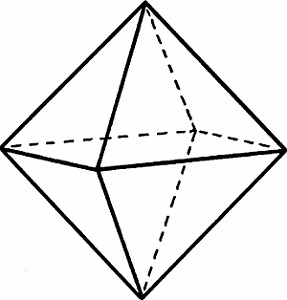
\includegraphics[width=0.25\textwidth]{images/octahedron.jpg}
    \caption{Triangulation of $\bbp^1$: the north pole is $\infty$, the south pole is $0$, ``the square equator" is the unit circle in $\bbc$.}
  \end{figure}

\end{qbox}

Using $\chi(X) = 2 - 2g(X)$, we can rewrite Theorem \ref{thm:RiemannHurwitz} as
  \begin{align*}
    g(X) - 1 = N \cdot (g(Y) - 1) + \sum_{i = 1}^k \left(\mathrm{index}_f(z_i) - 1\right) \cdot 1/2
  \end{align*}
  where $g$ is the genus.




  \begin{corollary}
    For a compact Riemann surface $Y$, there are no non-constant differentiable functions $f: \bbp^1 \rightarrow Y$ if $Y \not \cong \bbp^1$.
  \end{corollary}




\begin{corollary}
  If $X$ and $Y$ are complex tori (genus=1) then any non-constant complex differentiable map $f:X \rightarrow Y$ has no ramification points, i.e. the only maps between complex tori are (genuine) covering maps.
\end{corollary}

\begin{corollary}
  If $X$ and $Y$ are compact Riemann surfaces and there is a non-constant complex differentiable map $f:X \rightarrow Y$ which is not an isomorphism, then $g(X) \ge g(Y)$.
\end{corollary}

\begin{qbox}
  Prove the above corollaries using Theorem \ref{thm:RiemannHurwitz}.
\end{qbox}










\section{Elliptic curves}
  \emph{Analogy:} We can construct 1-dimensional real manifolds by looking at solutions to equations $f(x,y) = 0$ inside $\bbr^2$.

  We can do a similar thing for complex manifolds.
  Consider
  \begin{align*}
    S_p = \set{(z,w) : p(z,w) = 0} \subseteq \bbc^2
  \end{align*}

  Under certain restrictions on $p$, this defines a Riemann surface. In particular, this is true when $p(z,w) = z^2 - q(w)$ where $q(w)$ is a degree three polynomial with distinct roots. Further, it is possible to compactify this object by adding a single point at $\infty$ and the resulting object is called an \emph{elliptic curve}.
  \begin{align*}
    \cale ll_q = \set{(z,w) : z^2 = q(w) } \cup \set{\infty}
  \end{align*}

  There is a natural map
  \begin{align*}
    \cale ll_q &\longrightarrow \bbp^1 \\
    (z,w) &\longmapsto w \\
    \infty &\longmapsto \infty
  \end{align*}
  Turns out this is a complex differentiable map of degree 2 which has exactly 4 distinct ramification points, the three roots of $q$ and the point at infinity.
  Plugging in the Riemann--Hurwitz formula we get
  \begin{align*}
    \chi(\cale ll_q)
    &= 2 \chi(\bbp^1) \: + \sum_{\mbox{ 4 points}} (2 - 1) \\
    &= 4 - 4 \\
    &= 0
  \end{align*}
  Hence, $\cale ll_q$ is homeomorphic to a torus.

  \begin{mdframed}
    Almost nothing in this section generalizes arbitrarily.
    Not all compact Riemann surfaces can be embedded in $\bbp^2$, not all non-compact Riemann surfaces can be compactified by adding a single point at infinity.\\

    But things DO generalize with some effort. All compact Riemann surfaces can be embedded in $\bbp^3$, many non-compact Riemann surfaces of interest can be compactified by adding multiple points at infinity.
    It is a very non-trivial theorem in complex analysis that every Riemann surface admits a non-constant meromorphic function.\\

    It is a remarkable accident that things work out to be so nice for elliptic curves.\\

    We will make all of this rigorous (as much as possible) in the next two classes.
  \end{mdframed}
\end{document}
